%%%%%%%%%%%%%%%%%%%%%%%%%%%%%%%%%%%%%%%%%%%%%%%%%%%%%%%%%%%%%%%%%%%%%%%%%%%%%%%%
%%%%%%%%%%%%%%%%%%   Vorlage für eine Abschlussarbeit   %%%%%%%%%%%%%%%%%%%%%%%%
%%%%%%%%%%%%%%%%%%%%%%%%%%%%%%%%%%%%%%%%%%%%%%%%%%%%%%%%%%%%%%%%%%%%%%%%%%%%%%%%

% Erstellt von Maximilian Nöthe, <maximilian.noethe@tu-dortmund.de>
% ausgelegt für lualatex und Biblatex mit biber

% Kompilieren mit 
% lualatex dateiname.tex
% biber dateiname.bcf
% lualatex dateiname.tex
% lualatex dateiname.tex
% oder einfach mit:
% make

\documentclass[
  %tucolor,
  BCOR=12mm,     % 12mm binding corrections, adjust to fit your binding
  parskip=half,  % new paragraphs start with half line vertical space
  open=any,      % chapters start on both odd and even pages
  cleardoublepage=plain,  % no header/footer on blank pages
]{tudothesis}


% Warning, if another latex run is needed
\usepackage[aux]{rerunfilecheck}

% just list chapters and sections in the toc, not subsections or smaller
\setcounter{tocdepth}{1}

%------------------------------------------------------------------------------
%------------------------------ Sprache und Schrift: --------------------------
%------------------------------------------------------------------------------
\usepackage{fontspec}
\defaultfontfeatures{Ligatures=TeX}  % -- becomes en-dash etc.

% german language
\usepackage{polyglossia}
\setdefaultlanguage{english}

% for english abstract and english titles in the toc
\setotherlanguages{german}

% intelligent quotation marks, language and nesting sensitive
\usepackage[autostyle]{csquotes}

% microtypographical features, makes the text look nicer on the small scale
\usepackage{microtype}

%------------------------------------------------------------------------------
%------------------------ Für die Matheumgebung--------------------------------
%------------------------------------------------------------------------------

\usepackage{amsmath}
\usepackage{amssymb}
\usepackage{mathtools}

% Enable Unicode-Math and follow the ISO-Standards for typesetting math
\usepackage[
  math-style=ISO,
  bold-style=ISO,
  sans-style=italic,
  nabla=upright,
  partial=upright,
]{unicode-math}
\setmathfont{Latin Modern Math}

% nice, small fracs for the text with \sfrac{}{}
\usepackage{xfrac}  


%------------------------------------------------------------------------------
%---------------------------- Numbers and Units -------------------------------
%------------------------------------------------------------------------------

\usepackage[
  locale=DE,
  separate-uncertainty=true,
  per-mode=symbol-or-fraction,
]{siunitx}
\sisetup{math-micro=\text{µ},text-micro=µ}

%------------------------------------------------------------------------------
%-------------------------------- tables  -------------------------------------
%------------------------------------------------------------------------------

\usepackage{booktabs}       % stellt \toprule, \midrule, \bottomrule

%------------------------------------------------------------------------------
%-------------------------------- graphics -------------------------------------
%------------------------------------------------------------------------------

\usepackage{graphicx}
\usepackage{grffile}

% allow figures to be placed in the running text by default:
\usepackage{scrhack}
\usepackage{float}
\floatplacement{figure}{htbp}
\floatplacement{table}{htbp}

% keep figures and tables in the section
\usepackage[section, below]{placeins}


%------------------------------------------------------------------------------
%---------------------- customize list environments ---------------------------
%------------------------------------------------------------------------------

\usepackage{enumitem}

%------------------------------------------------------------------------------
%------------------------------ Bibliographie ---------------------------------
%------------------------------------------------------------------------------

\usepackage[
  backend=biber,   % use modern biber backend
  autolang=hyphen, % load hyphenation rules for if language of bibentry is not
                   % german, has to be loaded with \setotherlanguages
                   % in the references.bib use langid={en} for english sources
]{biblatex}
\addbibresource{references.bib}  % die Bibliographie einbinden
\DefineBibliographyStrings{german}{andothers = {{et\,al\adddot}}} 

%------------------------------------------------------------------------------
%------------------------------ Sonstiges: ------------------------------------
%------------------------------------------------------------------------------

\usepackage[pdfusetitle,unicode,linkbordercolor=tugreen]{hyperref}
\usepackage{bookmark}
\usepackage[shortcuts]{extdash}

%------------------------------------------------------------------------------
%-------------------------    Angaben zur Arbeit   ----------------------------
%------------------------------------------------------------------------------

\author{Marius Nagel}
\title{\boldmath Jet Cleaning Studies for Monotop Topologies at the ATLAS Detector at $\sqrt{s}=\SI{13}{\tera\electronvolt}$\unboldmath}
\date{2016}
\birthplace{Soest}
\chair{Lehrstuhl für Experimentelle Physik IV}
\division{Fakultät Physik}
\thesisclass{Bachelor of Science}
\submissiondate{31. September 2015}
\firstcorrector{Prof.~Dr.~Erstgutachter}
\secondcorrector{Prof.~Dr.~Zweitgutachter}

% tu logo on top of the titlepage

\titlehead{\includegraphics[height=1.5cm]{logos/tu-logo.pdf}
	\centering}


\begin{document}
\frontmatter
\thispagestyle{empty}
\setcounter{page}{2}
\section*{Hinweise}
Empfohlen wird die Verwendung dieser Vorlage mit der jeweils aktuellsten TeXLive Version (Linux, Windows) bzw. MacTeX Version (MacOS).
Aktuell ist dies TeXLive 2015. Download hier:
\begin{center}
  \ttfamily\url{https://www.tug.org/texlive/}
\end{center}
Bei Verwendung von TexLive Versionen 2014 und älter sollte
die Zeile
\begin{center}
\verb+\RequirePackage{fixltx2e}+ 
\end{center}
als erste Zeile der Präambel noch vor der Dokumentenklasse eingefügt werden.
Dies lädt diverse Bugfixes für LaTeX, die ab TexLive 2015 Standard sind.

Die Vorlage \texttt{thesis.tex} ist für die Kompilierung mit \texttt{lualatex} ausgelegt, mit wenigen Anpassungen kann sie aber auch mit \texttt{pdflatex} oder \texttt{xelatex} verwendet werden. 
Die Dokumentenklasse \texttt{tudothesis.cls} kann mit allen drei Programmen verwednet werden.

Achten Sie auch auf die Kodierung der Quelldateien.
Bei Verwendung von Xe\LaTeX\ oder Lua\LaTeX\ (empfohlen) müssen die
Quelldateien UTF-8 kodiert sein.
Bei Verwendung von pdf\LaTeX\ nutzen Sie die Pakete \texttt{inputenc} und \texttt{fontenc} mit der korrekten Wahl der Kodierungen.

Eine aktuelle Version dieser Vorlage steht unter 
\begin{center}
  \ttfamily\url{https://github.com/maxnoe/tudothesis}
\end{center}
zur Verfügung.

Alle verwendeten Pakete werden im \LaTeX{} Kurs von Pep et al.\ erklärt:
\begin{center}
  \ttfamily\url{http://toolbox.pep-dortmund.org/notes}
\end{center}

Für Rückmeldungen und bei Problemen mit der Klasse oder Vorlage, bitte ein \emph{Issue} auf GitHub aufmachen oder eine Email an
\href{mailto:maximilian.noethe@tu-dortmund.de}{maximilian.noethe@tu-dortmund.de} schreiben.

Wenn Sie die Dokumentenklasse mit der Option \texttt{tucolor} laden, werden verschiedene Elemente in TU-Grün gesetzt.

\maketitle

% Gutachterseite
\makecorrectorpage

% hier beginnt der Vorspann, nummeriert in römischen Zahlen
\thispagestyle{plain}

\section*{Kurzfassung}
Hier steht eine Kurzfassung der Arbeit in deutscher Sprache inklusive der Zusammenfassung der
Ergebnisse.
Zusammen mit der englischen Zusammenfassung muss sie auf diese Seite passen.

\section*{Abstract}
\begin{english}
The abstract is a short summary of the thesis in English, together with the German summary it has to fit on this page.
\end{english}

\tableofcontents

\mainmatter
% Hier beginnt der Inhalt mit Seite 1 in arabischen Ziffern
%\chapter{Introduction}

\chapter{Monotop Topologies in Extensions of the Standard Model}

\section{Brief Introduction to the Standard Model of Particle Physics}
The Standard Model of Particle Physics is an extensive Theory, describing the known elementary particles and their fundamental interactions.
In the last 40 years the Standard Model has been continuously developed and has withstand many tests on its consistency.
Nevertheless there are physical phenomena which can not be described, as there is for example the gravitation.
The fundamental characteristics of elementary particles described by the Standard Model are mass, spin, electric and color charge.
The Standard Model includes two different types of elementary fermions as there are the leptons and the quarks containing each three particle generations.
The third type of particles are the gauge bosons.
The gauge bosons are mediating the fundamental interactions between the elementary particles.
The electromagnetic interaction is mediated by the photons, while the strong interaction is given by the gluon.
As the Leptons are not color charged they are excluded by the strong interaction.
The third fundamental interaction is the weak force which is given by the $\mathrm{Z^0}$, $\mathrm{W^+}$ and $\mathrm{W^-}$.
In contrast to the photon and the gluon, the gauge bosons for the weak interaction are massive.
In Addition there is the higgs boson with a spin 0 which is connected to the higgs mechanism which explaining the mass for the fermions and weak gauge bosons.
An Overview to the Standard Model particles is shown in figure \ref{}.

\section{Monotop Topologies in Proton-Proton Collisions}

In Theory there are many predictions for new kinds of particles.
One of these new particles types of particles are the so called "Vector Like Quarks" .
These are heavy particles with special properties for strong interaction and higgs mechanism.
In the following there will be considered more special processes for vector like quarks.
Those processes are "montop" events, where a vector like quark is produced and then decaying into one single top quark and another invisible final state.
In this context "invisible" means that there are particles created which are not detectable and so cause large amounts of "Missing Transverse Energy" $E_{\text{T}}^{\text{miss}}$.
The $E_{\text{T}}^{\text{miss}}$ is the energy which is needed do fulfil the momentum conservation in the transverse plane.
The properties of $E_{\text{T}}^{\text{miss}}$ will be further explained in chapter 2.
In figure \ref{} is shown an exemplary feynman graph for a monotop process, where the vector like quark decays into a top quark and a $\mathrm{Z^0}$ boson.
The $\mathrm{Z^0}$ by itself then decays into two neutrinos which are responsible for the  $E_{\text{T}}^{\text{miss}}$.
\chapter{Presence of masked Modules at the ATLAS Detector}%\label{make}

\section{Overview of the ATLAS Detector}

In this section there will be given a short description of the structure of the ATLAS detector with a focus on the hadronic calorimeter system.
The ATLAS detector is a general purpose detector for high energy proton-proton collisions which is build up at the Large Hadron Collider (LHC) at CERN.
The LHC is a particle accelerator colliding protons with center of mass energies of currently \SI{13}{\tera\electronvolt} in RunII.
The overall structure of the ATLAS detector is cylinder symmetric around the beam axis and is build up in different layers from the inside to the outside.
The angle transverse to the beam axis is described as the azimuthal angle $\phi$ whereas the angle along the beam axis is described as the pseudorapidity $\eta$.
An overall cut-away view of the ATLAS detector is shown in figure \ref{ATLAS}.
\begin{figure}[H]
	\centering
	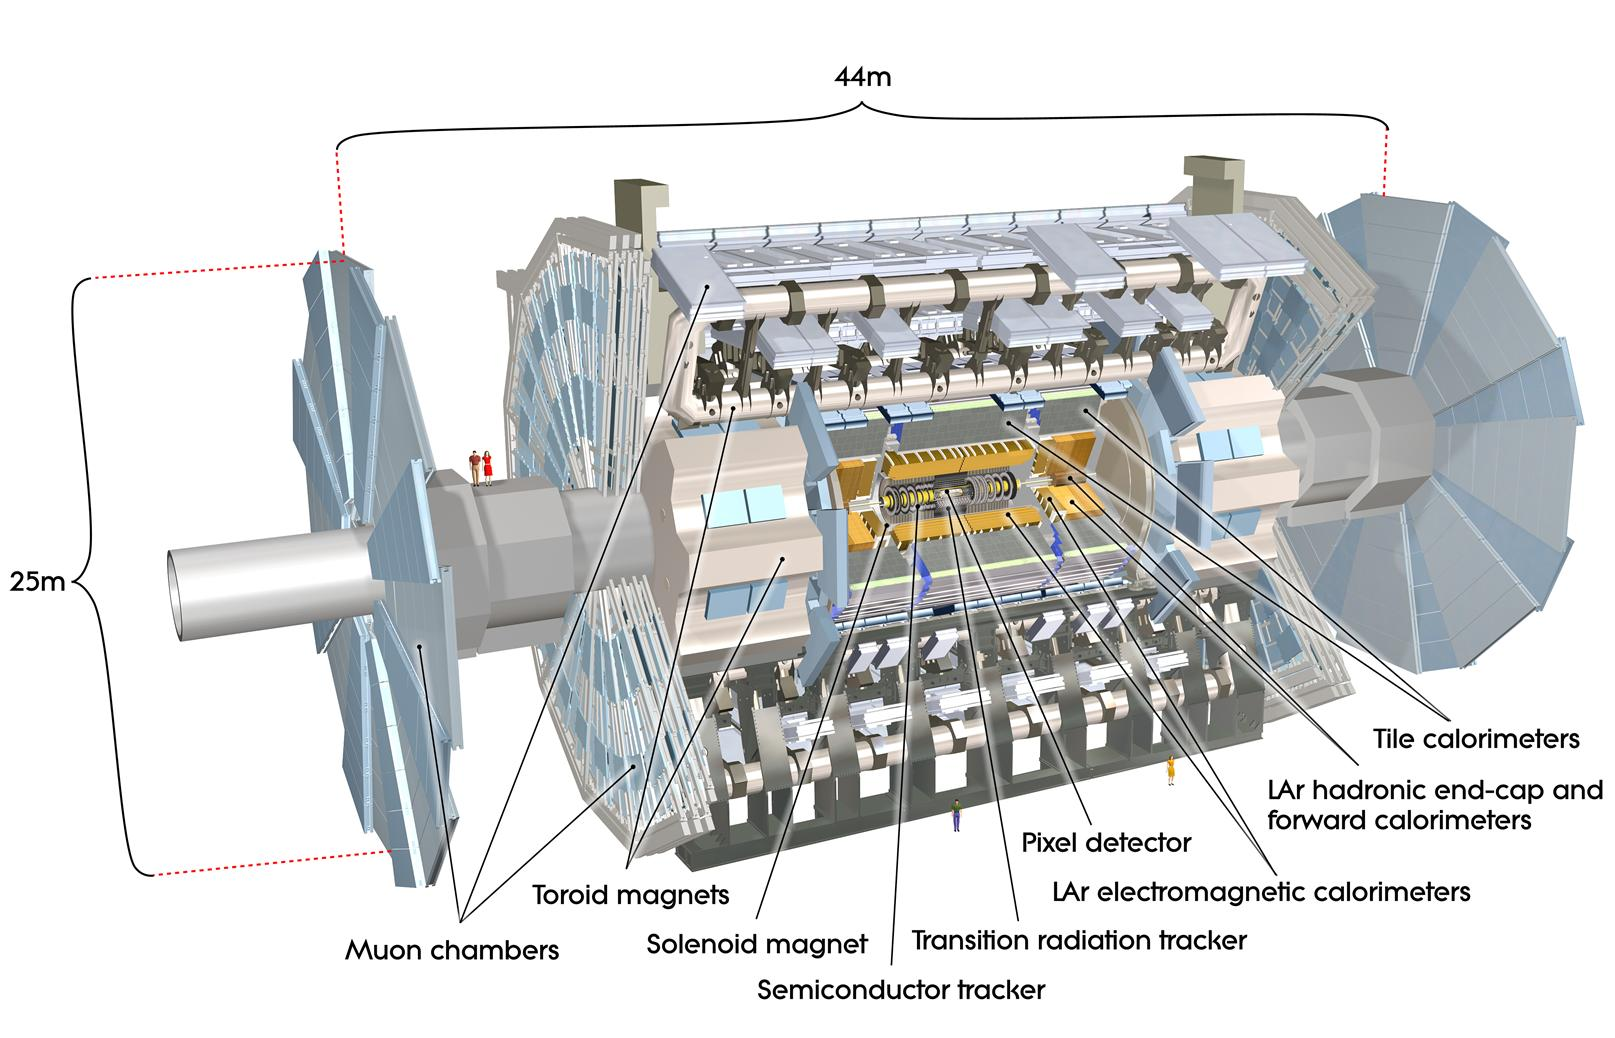
\includegraphics[width=\textwidth]{./Plots/figures_AtlasDetectorLabelled.png}
	\caption{Cut-away view of the ATLAS detector as detailed computer graphic.\cite{Aad:2008zzm}}
	\label{ATLAS}
\end{figure}
\subsection{The Inner Detector}
The innermost layer of the ATLAS detector is the Inner Detector (ID).
It is build by layers of silicon pixel and stripe detectors for precise measurements of particle tracks origin from the collision point.
The ID is permeated by a \SI{2}{\tesla} magnetic field for bending the charged particles track.
The track bending can be used for precise measurements of the momentum of charged particles.
In Addition the innermost layers of the ID can be used for vertex reconstruction.
The pixel and stripe detector systems cover in total a region of $|\eta| < 2.5$.
\subsection{Calorimeter Systems}
The calorimeter system of the ATLAS detector is build up in two layers and is designed to measure the energy deposits of hadronic and electromagnetic particles.
A cut-away view of the ATLAS calorimeter system is given in figure \ref{Calo}.
\begin{figure}[H]
	\centering
	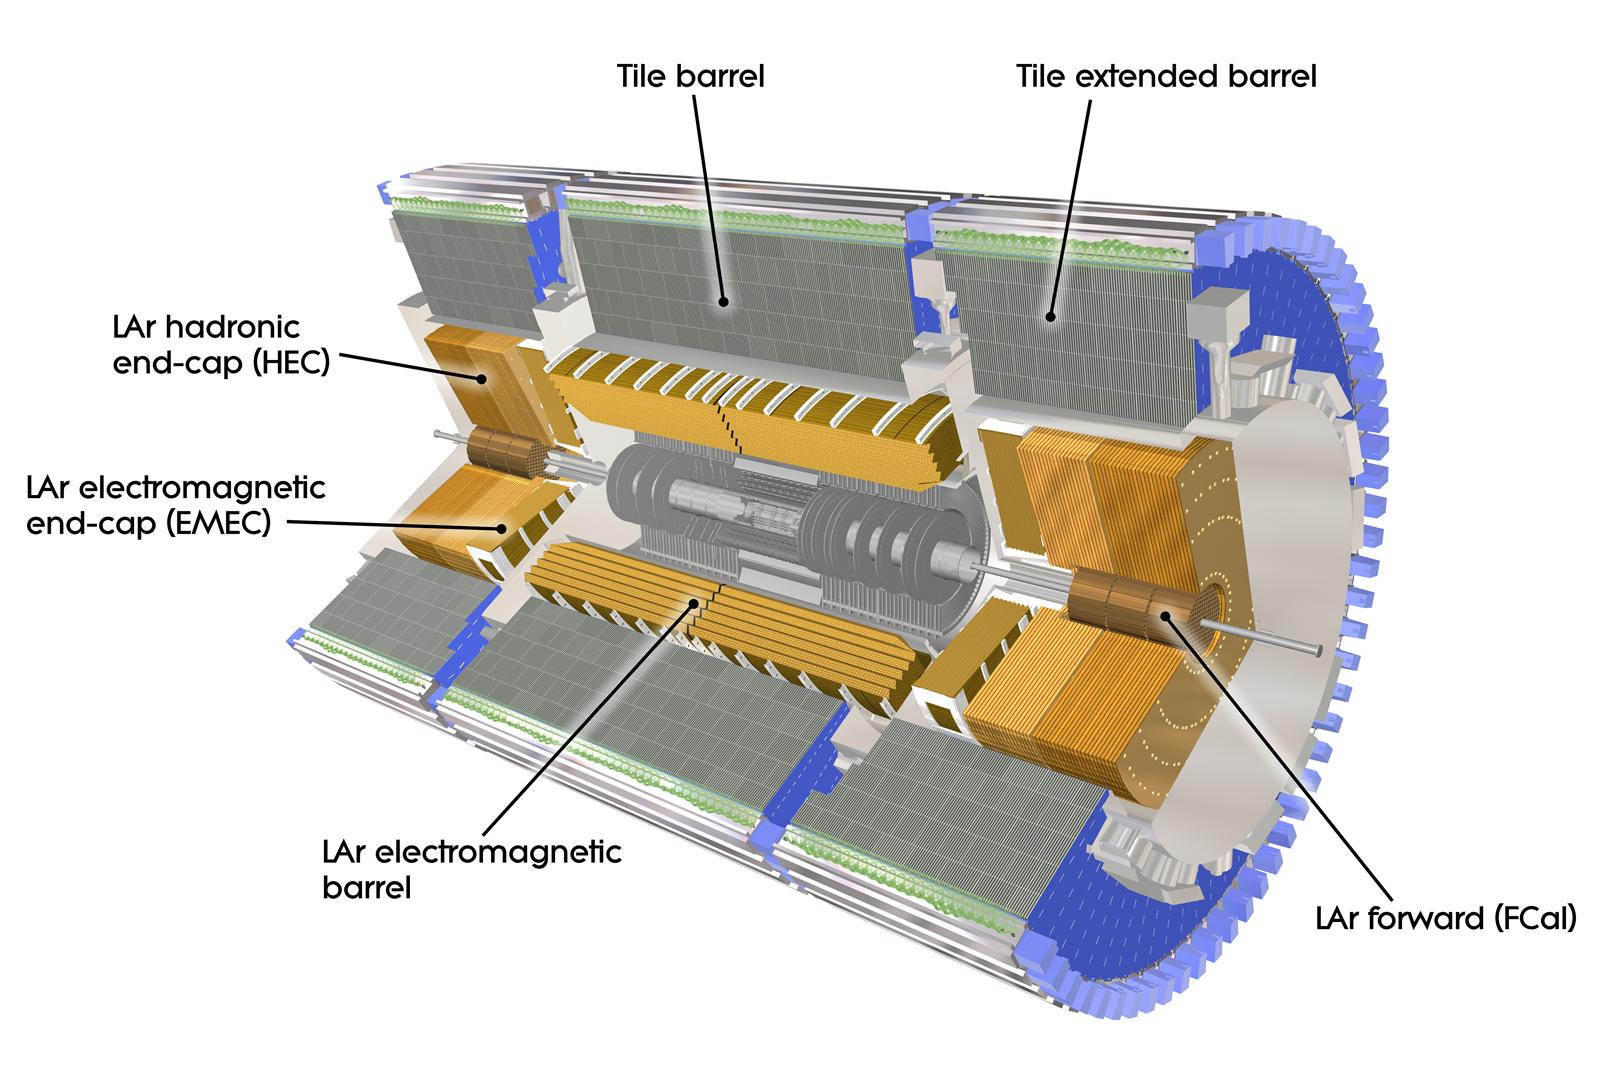
\includegraphics[width=\textwidth]{./Plots/atlas-calo-high.jpg}
	\caption{Cut-away view of the ATLAS calorimeter systems as detailed computer graphic.\cite{Aad:2008zzm}}
	\label{Calo}
\end{figure}
The inner layer of the calorimetry system is the liquid-argon electromagnetic calorimeter which covers in total a range of $|\eta| < 3.2$.
It is designed to absorb and measure most of the energy deposed by incoming electrons and photons but also detects energy depositions of hadronic particles.
The second layer of the calorimetry system is the hadronic calorimeter which is separated into a central barrel covering $|\eta| < 1$ and two extended barrels on the left and on the right of the detector covering each $0.8 < |\eta| < 1.7$.
The hadronic calorimeter is build as a sampling calorimeter and is constructed in layers of steel for energy absorption and scintillating material to measure the deposits.
Both electromagnetic and hadronic calorimeters also include forward calorimeters covering out wide regions in $|\eta|$.

As it is important for the following analysis, the specific segmentation of the hadronic calorimeter will be described here further.
The central barrel of the hadronic calorimeter is divided into two so called partitions LBA and LBC.
The LBC partition covers a region of $-1 < \eta < 0$ and the LBA partition covers $0 < \eta < 1$.
The extended barrels are each partitions called EBC and EBA, where EBC covers $-1.7 < \eta < -0.8$ and EBA $0.8 < \eta < 1.7$.
Each of this partitions is segmented into 64 modules in $\phi$, so that each module covers approximately a $\phi$ region of 0.1.
So the modules in the EBC for example are enumerated as EBC01 - EBC64.
\subsection{Myon System}
The outermost part of the ATLAS detector is the myon sytem for reconstruction of myon tracks.
Like the ID the myon system is permeated by a magnetic field to bend the tracks of the myons passing the detector.
\section{Jet and $\boldmath E_{\mathrm{T}}^{\mathrm{miss}}\unboldmath$ Reconstruction}
In proton-proton collisions various processes between elementary particles take place.
In many of this processes there are origin collimated "beams" of hadronic particles.
Those processes are called hadronisation processes and can be described with the strong interaction.
These "beams" are so called jets which are reconstructed as extended objects defined by their central axis position in the $\eta$-$\phi$-plane, their transverse momentum $p_{\text{T}}$ and their radius $\Delta R = \sqrt{\Delta\phi^2 + \Delta\eta^2}$.
So a jet can be characterised by specifying its four momentum and its $\Delta R$.

To reconstruct a jet with calorimeter informations, a jet clustering algorithm is needed.
The most commonly used algorithm is the anti-$k_{\text{T}}$ algorithm which is a subclass of the $k_{\text{T}}$ algorithms.
Those algorithms are able to identify clusters in the calorimeter systems to build up a jet.
For the anti-$k_{\text{T}}$ algorithm a $\Delta R$ can be given as an input parameter for the size of the jet.
In the following analysis there are two types jets given, the small-R jets with $\Delta R = 0.4$ and the large-R jets with $\Delta R = 1.0$.

In Addition the ID can be used to calibrate the reconstructed jets in the calorimeter, because the measured momentum in the ID is proportional to the energy measured by the calorimeter systems.
The requirement for this calibration is that the reconstructed jet lies inside of the acceptance of the ID, so that $|\eta|$ has to be smaller than 2.5 for small-R jets and 2.0 for large-R jets.

Another important factor for physics analysis is the Missing Transverse Energy $E_{\mathrm{T}}^{\mathrm{miss}}$.
This is the momentum which is missed to fulfil the momentum conservation in the transverse plane.
It should be mentioned that the momentum conservation can not be observed in the direction of $\eta$.
This is due to the fact, that the proton consists of many constituents colliding individually, so that the initial momentum can not be observed.
$E_{\mathrm{T}}^{\mathrm{miss}}$ can be caused by real physics objects which are not observable by the detector like neutrinos or undiscovered particles.
However $E_{\mathrm{T}}^{\mathrm{miss}}$ can be increased or even decreased by conditions like failed reconstructions or even masked regions in the detector, as it will be described in the further section.
Mathematically the $E_{\mathrm{T}}^{\mathrm{miss}}$ is defined as the negative vectorial sum of transverse momenta  of all reconstructed objects:
\begin{equation}
\vec{E}_{\mathrm{T}}^{\mathrm{miss}} = -\sum_{\mathrm{all}} \vec{p}_{\text{T}}.
\end{equation}
The $E_{\mathrm{T}}^{\mathrm{miss}}$ can than be calculated by the absolute of $\vec{E}_{\mathrm{T}}^{\mathrm{miss}}$.

\section{Effects of masked Calorimeter Modules}
As currently identified, there a two modules at the ALTAS detector which are permanently masked.
These are the LBA10 and the EBC21 modules in the hadronic calorimeter.
In figure \ref{masked_modules} a $\eta$-$\phi$-map shows the regions for which small-R jets can be affected by the masked modules.
\begin{figure}[H]
	\centering
	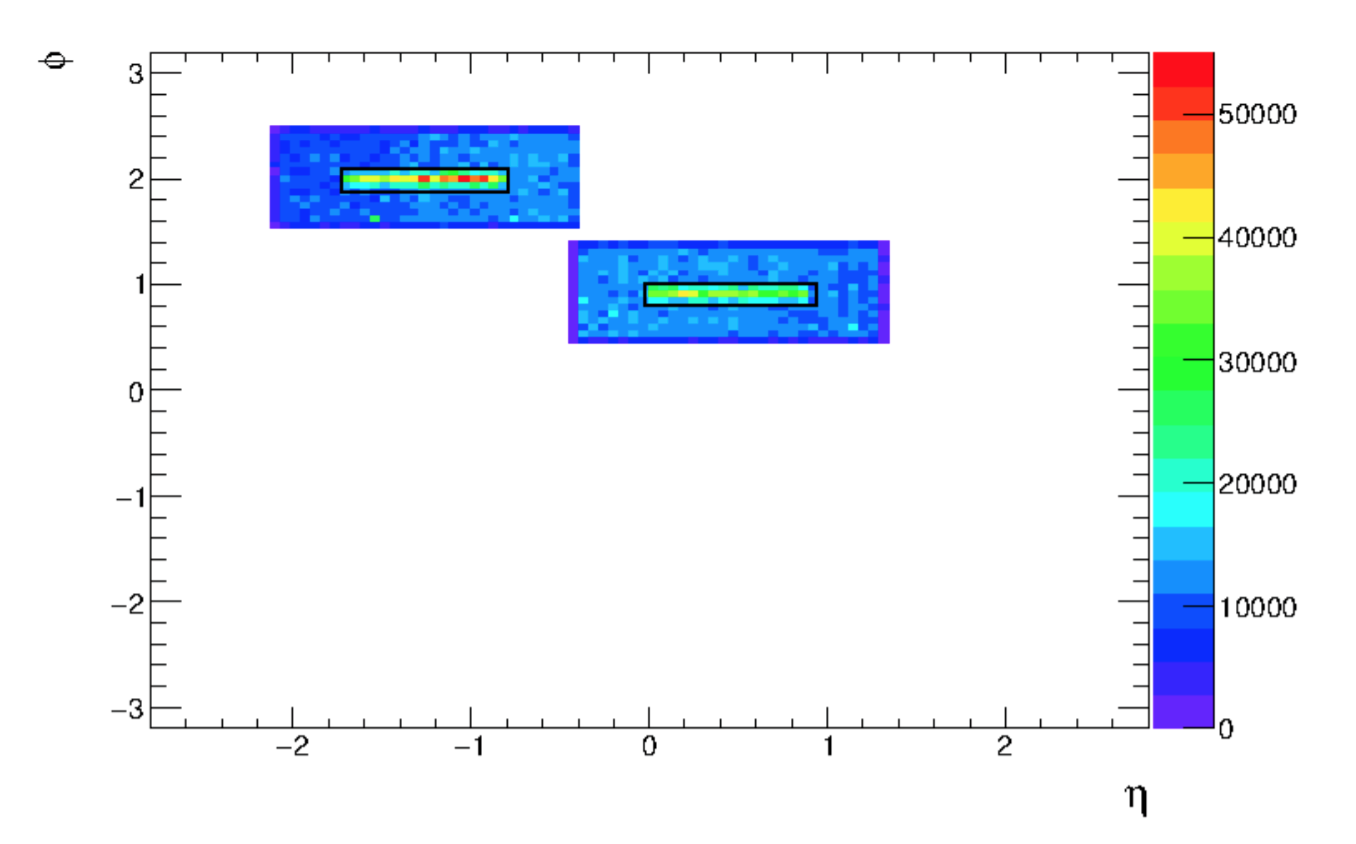
\includegraphics[width=\textwidth]{./Plots/Masked_map.png}
	\caption{$\eta-\phi$-map of small-R jets affected by the masked modules. The inner squares show the regions where the masked modules are.\cite{RodriguezPerez:2126928}}
	\label{masked_modules}
\end{figure}
Jets which are pointing right into the masked modules or close enough to them will be critical miss measured in $p_{\text{T}}$.
This can be especially a source of large $E_{\mathrm{T}}^{\mathrm{miss}}$ and so be critical for processes where large $E_{\mathrm{T}}^{\mathrm{miss}}$ is expected.
As the the modules affect jets in extended regions of $\eta$ and $\phi$, the jet reconstruction will be affected, too.
So it is plausible, that the jets affected by the masked modules will be also miss measured in $\eta$ and $\phi$.

As there are large amounts of $E_{\mathrm{T}}^{\mathrm{miss}}$ in potential monotop events, it is crucial to understand the effects of the masked modules. 
In figure \ref{Phi} are the $\phi$ distributions of the leading large-R jet an $E_{\mathrm{T}}^{\mathrm{miss}}$ are given for monotop data.
\begin{figure}
	\centering
	\begin{subfigure}{0.45\textwidth}
		\includegraphics[width=\textwidth]{./Plots/METphi2_.pdf}
		\caption{Phi distribution of $E_{\mathrm{T}}^{\mathrm{miss}}$ for montotop data.}
	\end{subfigure}
	\begin{subfigure}{0.45\textwidth}
		\includegraphics[width=\textwidth]{./Plots/fatjetphi_.pdf}
		\caption{Phi distribution of leading large-R jets for monotop data.}
	\end{subfigure}
	\caption{}\label{Phi}
\end{figure}
For the $\phi$ distribution of $E_{\mathrm{T}}^{\mathrm{miss}}$ there are two clear peaks positioned right at the position of the masked modules, where the left peak is on the position of LBA10 and the right peak on the position of EBC21.
The peaks in the leading large-R jet $\phi$ distribution are in the opposite $\phi$ direction compared to the $E_{\mathrm{T}}^{\mathrm{miss}}$ $\phi$ distribution. 

\section{JetTileCorrectionTool}
The JetTileCorrectionTool is a Tool which has been developed to correct the effect of masked calorimeter modules on the jet $p_{\text{T}}$ \cite{RodriguezPerez:2126928}.
It supplies the correction by the commonly used technique of inversion of the response function $\mathcal{R}$ \cite{Aad:2014bia}, \cite{LopezMateos:1201006}, \cite{Marshall:1111434}.
The response function is defined as
\begin{equation}
	\mathcal{R}(p_{\text{T}}^{\text{healthy}}) = \frac{p_{\text{T}}^{\text{damaged}}}{p_{\text{T}}^{\text{healthy}}},
\end{equation}
where $p_{\text{T}}^{\text{healthy}}$ and $p_{\text{T}}^{\text{damaged}}$ are generated by MC samples.
The $p_{\text{T}}^{\text{healthy}}$ is created by simulating the ideal detector without masked modules and the $p_{\text{T}}^{\text{damaged}}$ is created by simulating the real detector hence including the masked modules.
Basically for the inversion method
\begin{equation}
\mathcal{R}(p_{\text{T}}^{\text{healthy}}) = \left< \frac{p_{\text{T}}^{\text{damaged}}}{p_{\text{T}}^{\text{healthy}}}\right>
\end{equation}
is calculated.
From that
\begin{equation}
	\mathcal{R}(p_{\text{T}}^{\text{damaged}}) = \frac{p_{\text{T}}^{\text{healthy}}}{p_{\text{T}}^{\text{damaged}}}	
\end{equation}
can be approximated by calculating
\begin{equation}
	p_{\text{T}}^{\text{damaged}} \approx \mathcal{R}(p_{\text{T}}^{\text{healthy}}) p_{\text{T}}^{\text{healthy}}.
\end{equation}
The thus obtained $\mathcal{R}(p_{\text{T}}^{\text{damaged}})$ can be used to correct the reconstructed jet $p_{\text{T}}$ from data by multiplication.
The extent of the correction is calculated depending on the distance of the jet to the masked module.
Currently the correction is only supplied for small-R jets.
Since there is no overlap of the influenced areas for small-R jets, the correction can be separately calculated for the EBC21 and LBA10 module.
The JetTileCorrectionTool decides whether a jet is influenced by the masked modules and categorizes it into three categories:
\begin{itemize}
\item JetTileStatus == 0: Jet is not affected and does not require a correction
\item JetTileStatus == 1: Jet is affected but can be corrected
\item JetTileStatus == 2: Jet is core affected and has to be rejected
\end{itemize}
In the following the JetTileStatus will be abbrevated as TS.

\chapter{Effect of Vetoing the masked Regions}%\label{make}

\section{Monotop Event Selection}

\section{Performance of different Options}
\chapter{Application of the JetTileCorrectionTool}

\section{Influence of the Correction on Jet $p_{\mathrm{T}}$}

\section{Propagation of the Correction to $E_{\mathrm{T}}^{\mathrm{miss}}$}

\section{Jet $p_{\mathrm{T}}$ Resolution Studies}
\chapter{Conclusions}%\label{make}

\appendix
% Hier beginnt der Anhang, nummeriert in lateinischen Buchstaben
%\chapter{Ein Anhangskapitel}

Hier könnte ein Anhang stehen, falls Sie z.B. Code, Konstruktionszeichnungen oder ähnliches mit in die Arbeit bringen wollen. Im Normalfall stehen jedoch alle Ihre Resultate im Hauptteil der Bachelorarbeit und ein Anhang ist überflüssig.


%\backmatter
\printbibliography

\cleardoublepage
\thispagestyle{empty}
\section*{Eidesstattliche Versicherung}
Ich versichere hiermit an Eides statt, dass ich die vorliegende Abschlussarbeit mit dem Titel \enquote{\thetitle} selbstständig und ohne unzulässige fremde Hilfe erbracht habe.
Ich habe keine anderen als die angegebenen Quellen und Hilfsmittel benutzt, sowie wörtliche und sinngemäße Zitate kenntlich gemacht. 
Die Arbeit hat in gleicher oder ähnlicher Form noch keiner Prüfungsbehörde vorgelegen.

\vspace*{1cm}\noindent
\begin{center}
  \begin{tabular}{@{}p{0.4\textwidth}@{\hspace{0.15\textwidth}}p{0.4\textwidth}@{}}
  \rule{\linewidth}{0.25pt}& \rule{\linewidth}{0.25pt}\\
  Ort, Datum & Unterschrift
  \end{tabular}
\end{center}

\subsection*{Belehrung}
Wer vorsätzlich gegen eine die Täuschung über Prüfungsleistungen betreffende Regelung einer Hochschulprüfungsordnung verstößt, handelt ordnungswidrig.
Die Ordnungswidrigkeit kann mit einer Geldbuße von bis zu \SI[round-mode=places, round-precision=2]{50000}{€} geahndet werden. 
Zuständige Verwaltungsbehörde für die Verfolgung und Ahndung von Ordnungswidrigkeiten ist der Kanzler/die Kanzlerin der Technischen Universität Dortmund. 
Im Falle eines mehrfachen oder sonstigen schwerwiegenden Täuschungsversuches kann der Prüfling zudem exmatrikuliert werden \mbox{(\S\,63 Abs. 5 Hochschulgesetz --HG--).}

Die Abgabe einer falschen Versicherung an Eides statt wird mit Freiheitsstrafe bis zu 3 Jahren oder mit Geldstrafe bestraft.

Die Technische Universität Dortmund wird ggf.\ elektronische Vergleichswerkzeuge (wie z.\,B.\ die Software \enquote{turnitin}) zur Überprüfung von Ordnungswidrigkeiten in Prüfungsverfahren nutzen. \\[\baselineskip]

\noindent Die oben stehende Belehrung habe ich zur Kenntnis genommen.\\[1cm]
\begin{center}
\begin{tabular}{@{}p{0.4\textwidth}@{\hspace{0.15\textwidth}}p{0.4\textwidth}@{}}
\rule{\linewidth}{0.25pt}& \rule{\linewidth}{0.25pt}\\
Ort, Datum & Unterschrift
\end{tabular}
\end{center}

\end{document}
